%%%%%%%%%%%%%%%%%%%%%%%%%%%%%%%%%%%%%%%%%%%%%%%%%%%%%%%%%%%%%%%%%%%%%%%%%%%%%%%%
%
% \chapter{Electromagnetic theory}\label{chEMTheory}
%
%%%%%%%%%%%%%%%%%%%%%%%%%%%%%%%%%%%%%%%%%%%%%%%%%%%%%%%%%%%%%%%%%%%%%%%%%%%%%%%%

This chapter briefly reviews the portions of the electromagnetic theory that are used in ERMES 20.0. For a more detailed information on the fundamentals of electromagnetic theory, look at the references \cite{Jackson, Griffiths, ProperTheory, LorrainCorson, Stratton, WangsnessIng, Ritz-MilfordIng}. For more advanced topics and specific applications in frequency domain, look at the references \cite{Balanis, HarringtonTime-Harmonic, Cessenat}.

\section{Maxwell's equations}

In the second half of the 19th century James Clerk Maxwell established in \cite{OriginalMaxwell, TreatiseMaxwell} a set of twenty equations with twenty unknowns that summarized all the electromagnetic phenomena known in those days. This set of equations was later reduced by Oliver Heaviside \cite{HeavisideMaxwell, HeavisideBio}, who simplified and transformed the original set with the help of the vector notation developed by himself concurrently with Josiah Willard Gibbs \cite{GibbsVectors, GibbsBio}. The term \emph{Maxwell's equations} is nowadays applied to the simplified version due to Heaviside:
\\[-1.5em]
\begin{eqnarray}
    \nabla\cdot\mathbf{D} &=& \rho, \label{MaxwellDivD}
	\\\nonumber
	\\[-0.25em]
	\nabla\times\mathbf{H} - \frac{\partial\mathbf{D}}{\partial{t}}
	&=& \mathbf{J}, \label{MaxwellRotH}
	\\\nonumber
	\\[-0.25em]
	\nabla\times\mathbf{E} + \frac{\partial\mathbf{B}}{\partial{t}}
	&=& 0, \label{MaxwellRotE}
	\\\nonumber
	\\[-0.25em]
	\nabla \cdot \mathbf{B} &=& 0, \label{MaxwellDivB}
\end{eqnarray}
where the vector functions \textbf{E}, \textbf{D}, \textbf{B} and \textbf{H} are usually called (although there is no universal agreement and different names can be found in the literature):
\begin{itemize}
	\itemsep0em 
	\item[]\textbf{E}: electric field $\left(volt/meter\right)$,
	\item[]\textbf{D}: electric displacement field $\left(coulomb/meter^{2}\right)$,
	\item[]\textbf{B}: magnetic flux density (also magnetic induction) $\left(tesla\right)$,
	\item[]\textbf{H}: magnetic field $\left(ampere/meter\right)$.
\end{itemize}
The sources that generate these electromagnetic fields are:
\begin{itemize}
	\itemsep0em 
	\item[]\textbf{J}: electric current density $\left(ampere/meter^{2}\right)$,
	\item[]$\rho$: electric charge density $\left(coulomb/meter^{3}\right)$,
\end{itemize}
which are related through the continuity equation
\begin{equation}\label{ContinuityEquation}
	\nabla\cdot\mathbf{J} + \frac{\partial\rho}{\partial{t}} = 0.
\end{equation}
The above relation express the law of conservation of charge. This law can be deduced from equations \eqref{MaxwellRotH} and \eqref{MaxwellDivD} using the fact that, for any vector function \textbf{F}, it is satisfied:
\begin{equation}\label{DivCurleq0}
	\nabla\cdot(\nabla\times\textbf{F}) = 0.
\end{equation}
The symbols $\nabla\cdot$ and $\nabla\times$ correspond to the divergence and the curl, respectively. The divergence is defined by
\begin{equation}\label{DefDiv}
	\nabla\cdot\mathbf{F} \equiv \lim_{V \rightarrow 0} \frac{1}{V}
	\oint_{S} \mathbf{F}\cdot\mathbf{\hat{n}} \; dS,
\end{equation}
where \textbf{F} is a vector function, \textit{V} is an arbitrary volume, \textit{S} is the surface surrounding that volume and, the integral is a surface integral with $\mathbf{\hat{n}}$ being the outward normal to the
surface \textit{S}. In cartesian coordinates, with $\mathbf{F} = F_{x}\mathbf{\hat{x}} + F_{y}\mathbf{\hat{y}} + F_{z}\mathbf{\hat{z}}$, the divergence takes the form:
\begin{equation}\label{CartesianDiv}
	\nabla\cdot\mathbf{F} = \frac{\partial F_{x}}{\partial x} + \frac{\partial F_{y}}{\partial y} + \frac{\partial F_{z}}{\partial z}.
\end{equation}
The curl in the direction given by the unit vector $\mathbf{\hat{n}}$ is defined by
\begin{equation}\label{DefRot}
	(\nabla\times\mathbf{F})\cdot\mathbf{\hat{n}}  \equiv \lim_{S \rightarrow 0} \frac{1}{S} \oint_{C} \mathbf{F}\cdot d\mathbf{r},
\end{equation}
where \textbf{F} is a vector function and the integral is a line integral along the boundary \textit{C} of the area \textit{S}. The area \textit{S} is perpendicular to $\mathbf{\hat{n}}$. In cartesian coordinates, with $\mathbf{F} = F_{x}\mathbf{\hat{x}} + F_{y}\mathbf{\hat{y}} + F_{z}\mathbf{\hat{z}}$, the curl takes the form:
\begin{equation}\label{CartesianRot}
	\nabla\times\mathbf{F} =    \left(\frac{\partial F_z}{\partial y} - \frac{\partial F_y}{\partial z}\right)\mathbf{\hat{x}} + \left(\frac{\partial F_x}{\partial z} - \frac{\partial F_z}{\partial x}\right)\mathbf{\hat{y}} + \left(\frac{\partial F_y}{\partial x} - \frac{\partial F_x}{\partial y}\right)\mathbf{\hat{z}}.
\end{equation}
In principle, it is assumed that the Maxwell's equations are always valid, and that, if a vector function satisfies them, it is a possible electromagnetic field. It must be remembered that the Maxwell's equations are the mathematical expression of thoroughly validated experimental results, that is:
\begin{itemize}
	\itemsep0em 
    \item[\eqref{MaxwellDivD}] summarizes Coulomb's law of forces plus the effects of matter,
	\item[\eqref{MaxwellRotH}] represents an extension of Ampere's circuital law,
	\item[\eqref{MaxwellRotE}] represents Faraday's law of induction,
	\item[\eqref{MaxwellDivB}] proclaims the non-existence of magnetic monopoles.
\end{itemize}
\newpage
\noindent Under these circumstances, Maxwell's equations can not be demonstrated, but its applicability can be verified experimentally. Therefore, as a result of an extensive experimental work, it is considered that these set of equations can be applied to almost all macroscopic situations and that they can be used as guiding principles in the same way as the conservation of energy or the conservation of the linear momentum are used.

\subsection{Lorentz force}

To complete the description of the electromagnetic phenomena, an additional law must be added. This law is called the \emph{Lorentz force law} and 
it relates electromagnetism with mechanics:
\begin{equation}
	\mathbf{f} = \rho\,(\mathbf{E} + \mathbf{v}\times\mathbf{B}), \label{LorentzForce}
\end{equation}
where \textbf{f} is the force density $\left(newton/meter^{3}\right)$, \textbf{v} is the velocity of the electric charge density $\left(meter/second\right)$ and $\times$ represents the cross product.

Using the continuity equation \eqref{ContinuityEquation}, it can be shown that an electric charge density $\rho$ moving at a velocity \textbf{v} satisfies:
\begin{equation}\label{Jrhov}
	\textbf{J} = \rho\,\textbf{v}.
\end{equation}
Therefore, the Lorentz force \eqref{LorentzForce} can also be written as:
\begin{equation}
	\mathbf{f} = \rho\,\mathbf{E} + \mathbf{J}\times\mathbf{B}, \label{LorentzForceJ}
\end{equation}
and the power per unit volume \emph{p} $\left(watt/meter^{3}\right)$ generated by this Lorentz force is
\begin{equation}
	\emph{p} = \mathbf{f}\cdot\mathbf{v} =  \rho\,(\mathbf{E} + \mathbf{v}\times\mathbf{B})\cdot\mathbf{v} = \mathbf{E}\cdot\mathbf{J}.\label{PowerLorentzForce}
\end{equation}

\subsubsection{Lorentz force acting on a charged particle}

The mathematical description of the electric charge density of a charged point particle is:
\begin{equation}
	\rho(\mathbf{r}) = q\,\delta(\mathbf{r}-\mathbf{r}_{0}),\label{chargeDensityParticle}
\end{equation}
where q is the total electric charge of the particle, $\delta(\mathbf{r}-\mathbf{r}_{0})$ is the Dirac's delta function, and $\mathbf{r}_{0}$ is the position of the particle. Using \eqref{chargeDensityParticle} and \eqref{LorentzForce}, the total force \textbf{F} $\left(newton\right)$ on a charged point particle can be written as:
\begin{equation}
	\mathbf{F} = q\,(\mathbf{E} + \mathbf{v}\times\mathbf{B}),\label{LorentzForceParticle}
\end{equation}

\subsection{Constitutive relations}\label{ConstitutiveRelationsTheory}

Maxwell's equations cannot be solved until the relations \textbf{D} = \textbf{D}[\textbf{E}, \textbf{B}] and \textbf{H} = \textbf{H}[\textbf{E}, \textbf{B}] are known. These connections are called \emph{constitutive relations} and can be expressed as:
\begin{equation}\label{ConstitutiveRelationDE}
	\mathbf{D} = \epsilon_{0}\mathbf{E} + \mathbf{P},
\end{equation}
\begin{equation}\label{ConstitutiveRelationBH}
	\mathbf{H} = \frac{1}{\mu_{0}}\mathbf{B} - \mathbf{M},
\end{equation}
where
\begin{itemize}
	\itemsep0em 
	\item[]\textbf{P}: polarization $\left(coulomb/meter^{2}\right)$,
	\item[]\textbf{M}: magnetization $\left(ampere/meter\right)$,
	\item[]$\epsilon_{0}$: vacuum permittivity $\left(\frac{1}{36\pi}\cdot10^{-9} farad/meter\right)$,
	\item[]$\mu_{0}$: vacuum permeability $\left(4\pi\cdot10^{-7} henry/meter\right)$.
\end{itemize}
The quantity \textbf{P} represents the macroscopically averaged electric dipole moment per unit volume of a material medium. The quantity \textbf{M} represents the macroscopically averaged magnetic dipole moment per unit volume of a material medium. Higher order multipole moments are negligible in most materials, therefore, the knowledge of \textbf{P} and \textbf{M} is usually enough to have a complete characterization of a macroscopic media from the standpoint of the electromagnetic theory. \textbf{P} and \textbf{M} are functions of the fields, position and time and can not be predicted by the macroscopic electromagnetic theory, but they are accepted as an external information. These relations can be very complex and its determination are left to the experiment or to be calculated theoretically from microscopic models.

To complete the description of matter we should add a third constitutive equation, \textbf{J} = \textbf{J}[\textbf{E}, \textbf{B}], which also has to be known experimentally, or theoretically, and represents the electric current density induced on the media.

\subsubsection{Material types in electromagnetism}\label{GConstitutiveRelations}

From the electromagnetic theory point of view, materials are classified depending on the form of its constitutive relations \textbf{D} = \textbf{D}[\textbf{E}, \textbf{B}], \textbf{H} = \textbf{H}[\textbf{E}, \textbf{B}] and \textbf{J} = \textbf{J}[\textbf{E}, \textbf{B}]. For instance, linear materials are those with a linear dependency between the fields, isotropic materials are those in which the directions of the field pairs \textbf{D}[\textbf{E}], \textbf{B}[\textbf{H}], and \textbf{J}[\textbf{E}] are aligned, homogeneous materials are those with constant properties over its volume, and so on. 

In ERMES 20.0 there are implemented two types of materials: isotropic homogeneous linear materials and cold plasma, being the cold plasma a type of inhomogeneous gyrotropic linear material. In the cold plasma model implemeted in ERMES, the field \textbf{D} is related with \textbf{E} through a position dependant 3x3 Hermitian tensor with off-diagonal complex conjugate terms. The cold plasma permittivity tensor is calculated from a given electron density distribution and a magnetic flux density following the equations provided in \cite{Swanson}.

\subsubsection{Linear isotropic materials}\label{ILConstitutiveRelations}

Inside a linear isotropic material (time-invariant and local in space) the constitutive relations have the general form \cite{Cessenat}:
\begin{eqnarray}
    \mathbf{D}(\mathbf{r},t) &=& \int^{\infty}_{-\infty} \epsilon(\mathbf{r},t')\mathbf{E}(\mathbf{r}, t-t') \, dt', \label{GeneralLinearDE}
    \\\nonumber
	\\[-0.25em]
	\mathbf{B}(\mathbf{r},t) &=& \int^{\infty}_{-\infty} \mu(\mathbf{r},t')\mathbf{H}(\mathbf{r}, t-t') \, dt', \label{GeneralLinearBH}
	\\\nonumber
	\\[-0.25em]
	\mathbf{J}(\mathbf{r},t) &=& \int^{\infty}_{-\infty} \sigma(\mathbf{r},t')\mathbf{E}(\mathbf{r}, t-t') \, dt', \label{GeneralLinearJE}
\end{eqnarray}
where $\epsilon$, $\mu$ and $\sigma$ are scalars functions denominated
\begin{itemize}
	\item[]$\epsilon$: electric permittivity $\left(farad/meter\right)$,
	\item[]$\mu$: magnetic permeability $\left(henry/meter\right)$,
	\item[]$\sigma$: electric conductivity $\left(siemens/meter\right)$.
\end{itemize}
The assumed time-invariant property reveals a non-instantaneous response of the material to an applied field. This property allows to express the linear constitutive relation by means of a convolution in time. The assumed locality in space is a valid approximation when the spatial variation of the applied fields has a scale that is large compared with the dimensions involved in the creation of the atomic or molecular polarization. For visible light, or electromagnetic radiation of longer wavelength, it is often permissible to neglect the non-locality in space \cite{Jackson}. For conductors or some plasmas, however, the presence of free charges with macroscopic mean free paths makes this assumption to break down at much lower frequencies.

The constitutive relations \eqref{GeneralLinearDE}-\eqref{GeneralLinearJE} can be reformulated in the frequency domain by means of the Fourier transform, obtaining
\begin{eqnarray}
    \mathbf{D}(\mathbf{r}, \omega) &=& \epsilon(\mathbf{r},\omega)\,\mathbf{E}(\mathbf{r},\omega), \label{FourierGeneralLinearDE}
    \\\nonumber
	\\[-0.25em]
	\mathbf{B}(\mathbf{r}, \omega) &=& \mu(\mathbf{r}, \omega)\,\mathbf{H}(\mathbf{r}, \omega),\label{FourierGeneralLinearBH}
	\\\nonumber
	\\[-0.25em]
	\mathbf{J}(\mathbf{r}, \omega) &=& \sigma(\mathbf{r}, \omega)\,\mathbf{E}(\mathbf{r}, \omega),\label{FourierGeneralLinearJE}
\end{eqnarray}
where $\mathbf{D}(\mathbf{r}, \omega)$, $\mathbf{B}(\mathbf{r}, \omega)$, $\mathbf{J}(\mathbf{r}, \omega)$, $\mathbf{E}(\mathbf{r}, \omega)$ and $\mathbf{H}(\mathbf{r}, \omega)$ are the Fourier transform in time of $\mathbf{D}(\mathbf{r},t)$, $\mathbf{B}(\mathbf{r},t)$, $\mathbf{J}(\mathbf{r},t)$, $\mathbf{E}(\mathbf{r},t)$ and $\mathbf{H}(\mathbf{r},t)$, respectively. Also, $\epsilon(\mathbf{r}, \omega)$, $\mu(\mathbf{r}, \omega)$ and $\sigma(\mathbf{r}, \omega)$ are the Fourier transform in time of $\epsilon(\mathbf{r},t)$, $\mu(\mathbf{r},t)$ and $\sigma(\mathbf{r},t)$, respectively. A linear isotropic material is completely characterized, from the standpoint of the macroscopic electromagnetic theory, when $\epsilon$, $\mu$ and $\sigma$ are known, either in time domain or in frequency domain. The Fourier transform definition used to transform \eqref{GeneralLinearDE}-\eqref{GeneralLinearJE} into \eqref{FourierGeneralLinearDE}-\eqref{FourierGeneralLinearJE} was:
\begin{equation}
	F(\omega) =\int^{\infty}_{-\infty} f(t)e^{-i\omega t} \, dt.\label{FourierTransformT}
\end{equation}

\section{Potentials}\label{sAVPotentials}

Using Helmholtz's theorem and the equations \eqref{MaxwellDivB} and \eqref{MaxwellRotE}, it can be shown that there exist a scalar function $\phi$, called the electric potential, and a vectorial
function \textbf{A}, called magnetic vector potential, such as
\begin{eqnarray} 
    \mathbf{B} &=& \nabla\times\mathbf{A}, 
    \label{DefAPotential}
	\\
	\mathbf{E} &=& -\nabla\phi - \frac{\partial\mathbf{A}}{\partial t}.
	\label{DefAScalarPotential}
\end{eqnarray}
By replacing the above equations into \eqref{MaxwellDivD} and \eqref{MaxwellRotH}, and considering the general expressions for the constitutive relations \eqref{ConstitutiveRelationDE} and \eqref{ConstitutiveRelationBH}, it is obtained:
\begin{eqnarray} 
	\nabla^{2}\phi + \frac{\partial}{\partial t} \nabla\cdot\mathbf{A} &=& - \frac{1}{\epsilon_{0}} \left(\rho - \nabla\cdot\mathbf{P}\right),
	\label{MaxwellEqScalarPotential}
	\\
	\nabla^{2}\mathbf{A} - \mu_{0}\epsilon_{0}\frac{\partial^{2}\mathbf{A}}{\partial t^{2}} - \nabla\left(\nabla\cdot\mathbf{A} + \mu_{0}\epsilon_{0}\frac{\partial\phi}{\partial t}\right) &=& - \mu_{0}\left(\mathbf{J} + \nabla\times\mathbf{M} + \frac{\partial\mathbf{P}}{\partial t}\right),
	\label{MaxwellEqVectorPotential}
\end{eqnarray}
where the operator $\nabla^{2}$, when applied to a scalar function in a cartesian coordinate system, is defined by:
\begin{equation}\label{LaplaceOperatorScalar}
	\nabla^{2}\phi = \frac{\partial^{2}\phi}{\partial x^{2}} + \frac{\partial^{2}\phi}{\partial y^{2}} + \frac{\partial^{2}\phi}{\partial z^{2}}
\end{equation}
and, when applied to a vectorial function in a cartesian coordinate system, is defined by:
\begin{equation}\label{LaplaceOperatorVectorial}
	\nabla^{2}\mathbf{A} = \nabla^{2}A_{x}\,\mathbf{\hat{x}} + \nabla^{2}A_{y}\,\mathbf{\hat{y}} + \nabla^{2}A_{z}\,\mathbf{\hat{z}}.
\end{equation}
Equations \eqref{MaxwellEqScalarPotential} and \eqref{MaxwellEqVectorPotential} plus the definitions \eqref{DefAPotential} and \eqref{DefAScalarPotential} are totally equivalent to the set of equations \eqref{MaxwellDivD}-\eqref{MaxwellDivB}. If \eqref{MaxwellEqScalarPotential} and \eqref{MaxwellEqVectorPotential} are solved then, the fields \textbf{E} and
\textbf{B} obtained with \eqref{DefAPotential} and \eqref{DefAScalarPotential} will automatically satisfy all the Maxwell's equations \eqref{MaxwellDivD}-\eqref{MaxwellDivB}.

There are different possible \textbf{A} and $\phi$ potentials which give the same \textbf{E} and \textbf{B}. In fact, if $\chi$ is an arbitrary scalar function, any potential of the form
\begin{eqnarray} 
	\mathbf{A}^{+} &=& \mathbf{A} + \nabla\chi, \label{PossibleA}
	\\
	\phi^{+} &=& \phi - \frac{\partial\chi}{\partial t},\label{PossibleScalar}
\end{eqnarray}
will give the same fields \textbf{E} and \textbf{B}. This happens because any scalar function $\chi$ fulfils: 
\begin{equation}\label{CurlGrad}
    \nabla\times\left(\nabla\chi\right) = 0,
\end{equation}
where the operator $\nabla$ represents a gradient which, in cartesian coordinates, is defined by:
\begin{equation}\label{LaplaceOperatorScalar}
    \nabla\chi = \frac{\partial\chi}{\partial x}\,\mathbf{\hat{x}}  + \frac{\partial\chi}{\partial y}\,\mathbf{\hat{y}}  + \frac{\partial\chi}{\partial z}\,\mathbf{\hat{z}}.
\end{equation}
To have a unique solution in \eqref{MaxwellEqScalarPotential} and \eqref{MaxwellEqVectorPotential}, an extra condition over \textbf{A} and $\phi$ must be imposed. This extra condition is call the \emph{gauge} and there are several options. The most used gauge conditions are the \emph{Coulomb gauge}:
\begin{equation}\label{CoulombGauge}
    \nabla\cdot\mathbf{A} = 0,
\end{equation}
and the \emph{Lorenz gauge} \cite{LorenzLorentz, LorenzLorentz2}:
\begin{equation}\label{LorentzGauge}
    \nabla\cdot\mathbf{A} + \mu_{0}\epsilon_{0}\frac{\partial\phi}{\partial t} = 0.
\end{equation}
In some situations, thanks to the gauge freedom, a suitable choice of the $\textbf{A}-\phi$ gauge can simplify noticeably equations \eqref{MaxwellEqScalarPotential}-\eqref{MaxwellEqVectorPotential} and make them easier to solve than the Maxwell's equations \eqref{MaxwellDivD}-\eqref{MaxwellDivB} themselves.

\section{Time-harmonic Maxwell's equations}\label{sEMTH}

Time-harmonic fields are steady-state sinusoidally time varying electromagnetic fields. In ERMES 20.0 time-harmonic fields are represented in phasor notation as:
\begin{eqnarray}
    \mathbf{E}\,(\mathbf{r},t) &=& Real\left[\mathbf{E}_{c}(\mathbf{r})e^{-i\omega t}\right],\label{Ephasor}
	\\\nonumber
	\\[-1em]
	\mathbf{D}(\mathbf{r},t) &=& Real\left[\mathbf{D}_{c}(\mathbf{r})e^{-i\omega t}\right],\label{Dphasor}
    \\\nonumber
	\\[-1em]
	\mathbf{B}(\mathbf{r},t) &=& Real\left[\mathbf{B}_{c}(\mathbf{r})e^{-i\omega t}\right],\label{Bphasor}
	\\\nonumber
	\\[-1em]
	\mathbf{H}(\mathbf{r},t) &=& Real\left[\mathbf{H}_{c}(\mathbf{r})e^{-i\omega t}\right],\label{Hphasor}
\end{eqnarray}
where $i = \sqrt{-1}$  is the imaginary unit, $e^{-i\omega t} = cos(\omega t)\,-\,i\,sin(\omega t)$ is the Euler's formula modified by a sign, $\omega$ is a positive real number, $Real[\,.\,]$ denotes the real part of the expression in brackets, and $\mathbf{E}_{c}(\mathbf{r})$, $\mathbf{D}_{c}(\mathbf{r})$, $\mathbf{B}_{c}(\mathbf{r})$ and $\mathbf{H}_{c}(\mathbf{r})$ are vector complex functions that only depend on position. It is also assumed a steady-state sinusoidal time dependance for the sources which, in phasor notation, are written as:
\begin{eqnarray}
    \mathbf{J}(\mathbf{r},t) &=& Real\left[\mathbf{J}_{c}(\mathbf{r})e^{-i\omega t}\right],\label{Jphasor}
	\\\nonumber
	\\[-1em]
	\rho(\mathbf{r},t) &=& Real\left[\rho_{c}(\mathbf{r})e^{-i\omega t}\right].\label{Qphasor}
\end{eqnarray}
If expressions \eqref{Ephasor}-\eqref{Qphasor} are substituted into equations \eqref{MaxwellDivD}-\eqref{MaxwellDivB}, it is obtained the so-called \emph{time-harmonic Maxwell's equations}: 
\begin{eqnarray}
    \nabla\cdot\mathbf{D}_{c}(\mathbf{r}) &=& \rho_{c}(\mathbf{r}), \label{MaxwellDivDFD}
	\\\nonumber
	\\[-1em]
	\nabla\times\mathbf{H}_{c}(\mathbf{r}) + i\omega\mathbf{D}_{c}(\mathbf{r}) &=& \mathbf{J}_{c}(\mathbf{r}), \label{MaxwellRotHFD}
	\\\nonumber
	\\[-1em]
	\nabla\times\mathbf{E}_{c}(\mathbf{r}) - i\omega\mathbf{B}_{c}(\mathbf{r}) &=& 0, \label{MaxwellRotEFD}
	\\\nonumber
	\\[-1em]
	\nabla\cdot\mathbf{B}_{c}(\mathbf{r}) &=& 0. \label{MaxwellDivBFD}
\end{eqnarray}
To reach these equations it was used the fact that, an arbitrary complex function $F_{c} = F_{r} + iF_{i}$, satisfies
\begin{equation}
    Real\left[F_{c}e^{-i\omega t}\right] = 0 \,\,\,\,\, \forall\,t \,\,\, \Leftrightarrow \,\,\, F_{r} = 0 \, , \, F_{i} = 0\label{RealCero}
\end{equation}
and
\begin{equation}
	\frac{\partial}{\partial t}\left( F_{c}e^{-i\omega t} \right) = -i\omega F_{c}e^{-i\omega t}.\label{PhasorTDerivative}
\end{equation}
The solutions of equations \eqref{MaxwellDivDFD}-\eqref{MaxwellDivBFD} are vector complex functions that depend exclusively on the position. The physical solution in time domain can be recovered using the expressions \eqref{Ephasor}-\eqref{Hphasor}:
\begin{equation}\label{Freal}
    \textbf{F}(\textbf{r},t) = Real\left[\left(\mathbf{F}_{r}(\textbf{r}\right) + i\,\mathbf{F}_{i}(\textbf{r}))e^{-i\omega t}\right] = \mathbf{F}_{r}(\textbf{r})\cos(\omega t) + \mathbf{F}_{i}(\textbf{r})\sin(\omega t),
\end{equation}
where $\mathbf{F}$ is any of the electromagnetic fields in \eqref{Ephasor}-\eqref{Hphasor}. The time average of the dot and cross product of the quantities $\mathbf{F}(\textbf{r},t) = Real\left[\mathbf{F}_{c}(\textbf{r})e^{-i\omega t}\right]$ and $\mathbf{G}(\textbf{r},t) = Real\left[\mathbf{G}_{c}(\textbf{r})e^{-i\omega t}\right]$ can be calculated using: 
\begin{eqnarray}
    \left\langle \,\, \textbf{F}(\textbf{r},t)\,\cdot\,\textbf{G}(\textbf{r},t) \,\, \right\rangle &=& \frac{1}{T}\int^{T}_{0} \textbf{F}(\textbf{r},t)\,\cdot\,\textbf{G}(\textbf{r},t) \,\, dt = \frac{1}{2} \,\, Real\left[\textbf{F}_{c}(\textbf{r})\,\cdot\,\mathbf{\bar{G}}_{c}(\textbf{r})\right],\label{AverageTimeFdotG}
	\\\nonumber
	\\[-0.25em]
	\left\langle \,\, \textbf{F}(\textbf{r},t)\times\textbf{G}(\textbf{r},t) \,\, \right\rangle &=& \frac{1}{T}\int^{T}_{0} \textbf{F}(\textbf{r},t)\times\textbf{G}(\textbf{r},t) \,\, dt = \frac{1}{2} \,\, Real\left[\textbf{F}_{c}(\textbf{r})\times\mathbf{\bar{G}}_{c}(\textbf{r})\right],\label{AverageTimeFcrossG}
\end{eqnarray}
being $\mathbf{\bar{G}}_{c}$ the complex conjugate of $\textbf{G}_{c}$ and $T = 2\pi/\omega$ the period. For the specific case where $\textbf{F}_{c} = \textbf{G}_{c}$, expression \eqref{AverageTimeFdotG} can be simplified to:
\begin{equation}\label{AverageTimeFdotF}
    \left\langle \,\, \textbf{F}(\textbf{r},t)\cdot\textbf{F}(\textbf{r},t) \,\, \right\rangle = \left\langle \,\, |\,\textbf{F}(\textbf{r},t)\,|^{2} \, \right\rangle = \frac{1}{2} \,\, \textbf{F}_{c}(\textbf{r})\cdot\mathbf{\bar{F}}_{c}(\textbf{r}) = \frac{1}{2} \,\, |\,\textbf{F}_{c}(\textbf{r})\,|^{2}.
\end{equation}

\subsection{Time-harmonic Maxwell's equations in linear isotropic media}\label{MaxwellFD-LIM}

Inside a linear isotropic material (time-invariant and local in space) the constitutive relations have the general form given in \eqref{GeneralLinearDE}-\eqref{GeneralLinearJE}. Assuming the presence of time-harmonic electromagnetic fields as given in \eqref{Ephasor}-\eqref{Hphasor}, the constitutive relations \eqref{GeneralLinearDE}-\eqref{GeneralLinearJE} can be written as:
\begin{eqnarray}
    \mathbf{D}_{c}\left(\mathbf{r}\right) &=& \epsilon_{c}\left(\mathbf{r}\right)\,\, \mathbf{E}_{c}\left(\mathbf{r}\right), \label{ConstitutiveRelationDELFD}
	\\\nonumber
	\\[-1em]
	\mathbf{B}_{c}\left(\mathbf{r}\right) &=& \mu_{c}\left(\mathbf{r}\right)\, \mathbf{H}_{c}\left(\mathbf{r}\right),\label{ConstitutiveRelationBHLFD}
	\\\nonumber
	\\[-1em]
	\mathbf{J}_{c}\left(\mathbf{r}\right) &=& \sigma_{c}\left(\mathbf{r}\right)\,\, \mathbf{E}_{c}\left(\mathbf{r}\right),\label{ConstitutiveRelationJELFD}
\end{eqnarray}
where $\mathbf{E}_{c}$, $\mathbf{D}_{c}$, $\mathbf{B}_{c}$ and $\mathbf{H}_{c}$ are the complex valued vectorial functions defined in \eqref{Ephasor}-\eqref{Hphasor} and $\epsilon_{c}$, $\mu_{c}$ and $\sigma_{c}$ are the complex conjugate of the Fourier transform of the functions $\epsilon(\mathbf{r}, t)$, $\mu(\mathbf{r}, t)$ and $\sigma(\mathbf{r}, t)$ defined in \eqref{GeneralLinearDE}-\eqref{GeneralLinearJE}. In other words, if $\epsilon(\mathbf{r}, \omega)$, $\mu(\mathbf{r}, \omega)$ and $\sigma(\mathbf{r}, \omega)$ are the functions given in \eqref{FourierGeneralLinearDE}-\eqref{FourierGeneralLinearJE} and $\bar{\epsilon}(\mathbf{r}, \omega)$, $\bar{\mu}(\mathbf{r}, \omega)$ and $\bar{\sigma}(\mathbf{r}, \omega)$ are its complex
conjugates, then 
\begin{eqnarray}
    \epsilon_{c} &=& \bar{\epsilon}(\mathbf{r},\omega),\label{ExplainingFTEp}
	\\\nonumber
	\\[-1em]
	\mu_{c} &=& \bar{\mu}(\mathbf{r},\omega),\label{ExplainingFTMu}
	\\\nonumber
	\\[-1em]
	\sigma_{c} &=& \bar{\sigma}(\mathbf{r},\omega),\label{ExplainingFTSig}
\end{eqnarray}
where $\omega$ is the frequency at which the fields are oscillating. Since the response of materials to alternating fields is characterized by a complex value, we can separate its real and
imaginary parts in the following way:
\begin{eqnarray} 
    \epsilon_{c}\, &=&\, \epsilon^{'} + i \epsilon^{''},\label{complexPermittivity}
	\\\nonumber
	\\[-1em]
	\mu_{c} &=& \mu^{'} + i \mu^{''}, \label{ComplexPermeability}
	\\\nonumber
	\\[-1em]
	\sigma_{c} &=& \sigma^{'} + i \sigma^{''}.\label{ComplexConductivity}
\end{eqnarray}
The imaginary parts $\epsilon^{''}$ and $\mu^{''}$ and the real part $\sigma^{'}$ accounts for the dissipation (or loss) of energy within a medium. The real parts $\epsilon^{'}$ and $\mu^{'}$ and the imaginary part $\sigma^{''}$ are related to the stored energy within the medium.

The time-harmonic Maxwell's equations for linear isotropic media are obtained after substituting \eqref{ConstitutiveRelationDELFD}-\eqref{ConstitutiveRelationJELFD} into \eqref{MaxwellDivDFD}-\eqref{MaxwellDivBFD}:
\begin{eqnarray}
    \nabla\cdot\left(\epsilon_{c}\mathbf{E}_{c}\right) &=& \rho_{c}, \label{MaxwellDivDFDL}
	\\\nonumber
	\\[-1em]
	\nabla\times\mathbf{H}_{c} + i\omega\epsilon_{c}\mathbf{E}_{c} &=& \mathbf{J}_{c}, \label{MaxwellRotHFDL}
	\\\nonumber
	\\[-1em]
	\nabla\times\mathbf{E}_{c} - i\omega\mu_{c}\mathbf{H}_{c} &=& 0, \label{MaxwellRotEFDL}
	\\\nonumber
	\\[-1em]
	\nabla\cdot\left(\mu_{c}\mathbf{H}_{c}\right) &=& 0, \label{MaxwellDivBFDL}
\end{eqnarray}
where $\mathbf{E}_{c}$, $\mathbf{H}_{c}$, $\mathbf{J}_{c}$, $\rho_{c}$, $\epsilon_{c}$ and $\mu_{c}$ are complex valued functions that only depend on position. The term $\mathbf{J}_{c}$ in \eqref{MaxwellRotHFDL} includes all the \emph{free} current densities which are present in the problem domain. Free current densities are all the currents densities except those produced by the polarization and magnetization of the material. The currents densities produced by the polarization and magnetization of the material are implicit in $\epsilon_{c}$ and $\mu_{c}$. Free current densities are, for instance, the diffusion of charged particles, the induced eddy currents in conductive materials or, the impressed currents that are independent of the fields. Hence, we can write
\begin{equation}\label{CurrentDensitySplit}
    \mathbf{J}_{c} = \sigma_{c}\mathbf{E}_{c} + \mathbf{J}_{c}^{imp},
\end{equation}
where $\mathbf{J}_{c}^{imp}$ represents all the free current densities except those induced by the electric field in materials with conductivity. Substituting \eqref{CurrentDensitySplit} into \eqref{MaxwellRotHFDL} gives
\begin{equation}\label{MaxwellRotHFDLandSplitCurrent}
    \nabla\times\mathbf{H}_{c} + i\omega\left(\epsilon_{c} + i\, \frac{\sigma_{c}}{\omega}\right)\mathbf{E}_{c} = \mathbf{J}_{c}^{imp}.
\end{equation}
Applying the divergence to \eqref{MaxwellRotHFDLandSplitCurrent} and recalling \eqref{DivCurleq0}, equations \eqref{MaxwellDivDFDL}-\eqref{MaxwellDivBFDL} can be written as:
\begin{eqnarray}
    \nabla\cdot\left(\varepsilon_{c}\mathbf{E}_{c}\right) &=& \rho_{c}^{imp}, \label{MaxwellDivDFDLS}
	\\\nonumber
	\\[-1em]
	\nabla\times\mathbf{H}_{c} + i\omega\varepsilon_{c}\mathbf{E}_{c} &=& \mathbf{J}_{c}^{imp}, \label{MaxwellRotHFDLS}
	\\\nonumber
	\\[-1em]
	\nabla\times\mathbf{E}_{c} - i\omega\mu_{c}\mathbf{H}_{c} &=& 0, \label{MaxwellRotEFDLS}
	\\\nonumber
	\\[-1em]
	\nabla\cdot\left(\mu_{c}\mathbf{H}_{c}\right) &=& 0, \label{MaxwellDivBFDLS}
\end{eqnarray}
where
\begin{equation}\label{VarEpsilonDef}
    \varepsilon_{c} = \epsilon_{c} + i\, \frac{\sigma_{c}}{\omega} = \epsilon^{'} - \frac{\sigma^{''}}{\omega} + i\left(\epsilon^{''} + \frac{\sigma^{'}}{\omega}\right)
\end{equation}
and
\begin{equation}\label{ChargeDensityNC}
    \rho_{c}^{imp} = \frac{1}{i\omega}\nabla\cdot\mathbf{J}_{c}^{imp}.
\end{equation}
In equations \eqref{MaxwellDivDFDLS}-\eqref{MaxwellDivBFDLS} the effect of the induced currents are included in $\varepsilon_{c}$. On the other hand, in the equivalent set of equations \eqref{MaxwellDivDFDL}-\eqref{MaxwellDivBFDL}, the effect of the induced currents must be explicitly specify as shown in \eqref{CurrentDensitySplit}.

\section{Fields at the interface between two media}\label{sEMInterface}

When solving electromagnetic problems, it is usual to find materials with different electromagnetic properties in the domain under study. These properties are expected to change continuously (although abruptedly) in a narrow transition region between the two media. The assumption of a continuous change in the electromagnetic properties is made for consistency with the expected continuity of the physical fields and its derivatives. 

In general, the specific details of what actually happens in the transition layer between two media are not of interest. Therefore, it is customary to replace the real situation by an idealized one, in which, the width of the transition layer tends to zero and becomes a surface. Using the Maxwell's equations, it can be demonstrated that, at the interface between two media, the fields must satisfy the following discontinuity conditions:
\begin{eqnarray}
    \mathbf{\hat{n}}\,\cdot\,\left(\,\mathbf{D}_{1} - \mathbf{D}_{2}\,\right) &=& \rho_{s}, 
    \label{CondicionContornoDn}
	\\\nonumber
	\\[-1em]
	\mathbf{\hat{n}}\times\left(\,\mathbf{H}_{1} - \mathbf{H}_{2}\,\right) &=& \mathbf{J}_{s}, \label{CondicionContornoHt}
	\\\nonumber
	\\[-1em]
	\mathbf{\hat{n}}\times\left(\,\mathbf{E}_{1}\,-\,\mathbf{E}_{2}\,\right) &=& 0, 
	\label{CondicionContornoEt}
	\\\nonumber
	\\[-1em]
	\mathbf{\hat{n}}\,\cdot\,\left(\,\mathbf{B}_{1} - \mathbf{B}_{2}\,\right) &=& 0, 
	\label{CondicionContornoBn}
\end{eqnarray}
where $\mathbf{\hat{n}}$ is the unit normal of the idealized transition layer surface \emph{S} and it points from region 2 into region 1 (see Figure \ref{InterfaceBetweenMedia}). $\mathbf{J}_{s}$ and $\rho_{s}$ represent, respectively, a surface current density and a surface electric charge density located at \emph{S}. The fields $\mathbf{E}_{1}$, $\mathbf{D}_{1}$, $\mathbf{H}_{1}$ and $\mathbf{B}_{1}$ denotes the limiting values of the fields as \emph{S} is approached from region 1. Analogously, $\mathbf{E}_{2}$, $\mathbf{D}_{2}$, $\mathbf{H}_{2}$ and $\mathbf{B}_{2}$ denotes the limiting values of the fields as \emph{S} is approached from region 2. Expressions \eqref{CondicionContornoDn}-\eqref{CondicionContornoBn} are useful to connect solutions of the Maxwell's equations from different adjacent regions to obtain the fields in the entire domain of the problem.

Expressions \eqref{CondicionContornoDn}-\eqref{CondicionContornoBn} can be simplified with the help of \eqref{MaxwellDivDFDLS}-\eqref{MaxwellDivBFDLS} in the presence of linear isotropic materials and time-harmonic fields and sources: 
\begin{eqnarray}
    \mathbf{\hat{n}}\cdot\left(\varepsilon_{c_{1}}\mathbf{E}_{c_{1}} - \varepsilon_{c_{2}}\mathbf{E}_{c_{2}}\right) &=& \rho_{cs}^{imp}, \label{CondicionContornoDnLI}
	\\\nonumber
	\\[-1em]
    \mathbf{\hat{n}}\times\left(\mathbf{H}_{c_{1}} - \mathbf{H}_{c_{2}}\right) &=& \mathbf{J}_{cs}^{imp}, \label{CondicionContornoHtLI}
	\\\nonumber
	\\[-1em]
	\mathbf{\hat{n}}\times\left(\mathbf{E}_{c_{1}}\,-\,\mathbf{E}_{c_{2}}\right) &=& 0, \label{CondicionContornoEtLI}
	\\\nonumber
	\\[-1em]
	\mathbf{\hat{n}}\cdot\left(\mu_{c_{1}}\mathbf{H}_{c_{1}} - \mu_{c_{2}}\mathbf{H}_{c_{2}}\right) &=& 0, \label{CondicionContornoBnLI}
\end{eqnarray}
where $\varepsilon_{c_{1}}$ and $\mu_{c_{1}}$ are the complex permittivity and permeability of the material 1 as it is defined in \eqref{VarEpsilonDef} and \eqref{ConstitutiveRelationBHLFD}. Analogously, $\varepsilon_{c_{2}}$ and $\mu_{c_{2}}$ are the complex permittivity and permeability of the material 2. The complex vector functions $\mathbf{E}_{c_{1}}$ and $\mathbf{H}_{c_{1}}$, which are defined in \eqref{Ephasor} and \eqref{Hphasor}, denotes the limiting values of the fields as \emph{S} is approached from region 1. Similarly, $\mathbf{E}_{c_{2}}$ and $\mathbf{H}_{c_{2}}$ denotes the limiting values of the fields as \emph{S} is approached from region 2. $\mathbf{J}_{cs}^{imp}$ and $\rho_{cs}^{imp}$, which are defined in \eqref{CurrentDensitySplit} and \eqref{ChargeDensityNC}, represent, respectively, an imposed surface current density and an imposed surface electric charge density located at \emph{S}. 

In \eqref{CondicionContornoDnLI}-\eqref{CondicionContornoBnLI} it is not necessary to include explicitly the surface charge density and surface current density due to polarization, magnetization, and conductivity of the material. Their effects are implicit in the discontinuity of $\varepsilon_{c}$ and $\mu_{c}$. Only current densities or surface charge densities \textit{imposed} on the discontinuity surface and not coming from polarization, magnetization, and conductivity, need to be included through $\mathbf{J}_{cs}^{imp}$ and $\rho_{cs}^{imp}$.

\begin{figure}[h!]
	\begin{center}
		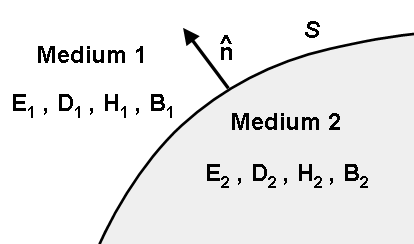
\includegraphics[width=0.60\textwidth]{Contents/Figures/EM-Interface.png}
		\caption{Fields at the interface \emph{S} between two media.}\label{InterfaceBetweenMedia}
	\end{center}
\end{figure}

\subsection{Perfect electric conductor}\label{sPECcond}

A \textit{Perfect Electric Conductor} (PEC) is a material in which the electric conductivity is considered infinite. A remarkable feature of this idealized material is that, in its interior, any time-harmonic field is zero. This can be seen, heuristically, using equations \eqref{ConstitutiveRelationJELFD} and \eqref{MaxwellRotEFDL} and assuming that, inside a PEC, the fields and the induced currents remain finite. 
From \eqref{ConstitutiveRelationJELFD}, if the conductivity is infinite, then $\mathbf{E}_{c}$ must vanish to have a finite $\mathbf{J}_{c}$. On the other hand, from \eqref{MaxwellRotEFDL}, if $\mathbf{E}_{c}$ is zero, then $\mathbf{H}_{c}$ must also be zero. 

For finite conductivity, linear isotropic materials, and time-harmonic regime, equations \eqref{CondicionContornoDnLI}-\eqref{CondicionContornoBnLI} can be deduced from \eqref{MaxwellDivDFDLS}-\eqref{MaxwellDivBFDLS}. In the case of an infinite conductivity, equations \eqref{MaxwellDivDFDL}-\eqref{MaxwellDivBFDL} must be used instead of \eqref{CondicionContornoDnLI}-\eqref{CondicionContornoBnLI} to obtain the PEC interface conditions:
\begin{eqnarray}
	\mathbf{\hat{n}}\cdot\varepsilon_{c_{1}}\mathbf{E}_{c_{1}}\, &=& \rho_{cs}, 
	\label{CondicionContornoDnLIPEC}
	\\\nonumber
	\\[-1em]
	\mathbf{\hat{n}}\times\mathbf{H}_{c_{1}} &=& \mathbf{J}_{cs}, 
	\label{CondicionContornoHtLIPEC}
	\\\nonumber
	\\[-1em]
	\mathbf{\hat{n}}\times\mathbf{E}_{c_{1}}\, &=& 0, 
	\label{CondicionContornoEtLIPEC}
	\\\nonumber
	\\[-1em]
	\mathbf{\hat{n}}\cdot\mu_{c_{1}}\mathbf{H}_{c_{1}} &=& 0, 
	\label{CondicionContornoBnLIPEC}
\end{eqnarray}
where the medium 2 of Figure \ref{InterfaceBetweenMedia} is considered the PEC. $\mathbf{J}_{cs}$ and $\rho_{cs}$ represent, respectively, a free surface current density and a free surface electric charge density imposed and confined in \emph{S}. 

An important characteristic behaviour of the fields on the surface of a PEC can be deduced from equations \eqref{CondicionContornoEtLIPEC} and \eqref{CondicionContornoBnLIPEC}. Outside a PEC, the electric field is normal to the surface \emph{S} and the magnetic field is tangential to surface \emph{S}.

\subsection{Imperfect electric conductor}\label{sIBCcond}

If the material 2 in Figure \ref{InterfaceBetweenMedia} is not a perfect conductor but it allows the fields to penetrate a small distance then, a time-harmonic electric field at \emph{S} satisfies approximately the relation \cite{Senior, SeniorLibro}:
\begin{equation}\label{ImperfectConductorE}
	\frac{1}{\mu_{c_{1}}}\mathbf{\hat{n}}\times\left(\nabla\times\mathbf{E}_{c_{1}}\right) + \left(i\omega\sqrt{\frac{\varepsilon_{c_{2}}}{\mu_{c_{2}}}}\right) \mathbf{\hat{n}}\times(\mathbf{\hat{n}}\times\mathbf{E}_{c_{1}}) = 0.
\end{equation}
Analogously, a time-harmonic magnetic field at \emph{S} satisfies approximately the relation:
\begin{equation}\label{ImperfectConductorH}
	\frac{1}{\varepsilon_{c_{1}}}\mathbf{\hat{n}}\times\left(\nabla\times\mathbf{H}_{c_{1}}\right) + \left(i\omega\sqrt{\frac{\mu_{c_{2}}}{\varepsilon_{c_{2}}}}\right)\mathbf{\hat{n}}\times\left(\mathbf{\hat{n}}\times\mathbf{H}_{c_{1}}\right) = 0.
\end{equation}
In the above expressions, the medium 2 of Figure \ref{InterfaceBetweenMedia} is considered the imperfect conductor, $\mathbf{E}_{c_{1}}$ and $\mathbf{H}_{c_{1}}$ denotes the limiting values of the fields as \emph{S} is approached from region 1, $\varepsilon_{c_{2}}$ and $\mu_{c_{2}}$ are the complex permittivity and permeability of the imperfect conductor and, $\varepsilon_{c_{1}}$ and $\mu_{c_{1}}$ are the complex permittivity and permeability of the material outside the imperfect conductor. The relations \eqref{ImperfectConductorE} and \eqref{ImperfectConductorH} are called \textit{Impedance Boundary Conditions} (IBC).

\section{Radiation condition}\label{sSMradcond}

A boundary condition at infinite must be specified on problems with unbounded domain to ensure the uniqueness of the solution of the time-harmonic Maxwell's equations \eqref{MaxwellDivDFDLS}-\eqref{MaxwellDivBFDLS} \cite{Cessenat}. Assuming all the sources and materials at a finite distance from the origin of coordinates and immersed in an infinite linear, isotropic, homogeneous, and lossless medium (characterize by the real parameters $\epsilon_{r}$ and $\mu_{r}$), the time-harmonic electric and magnetic fields must satisfy:
\begin{eqnarray}
    \lim_{r\rightarrow\infty} r \left[\nabla\times\mathbf{E}_{c}\,-\, i\omega\sqrt{\epsilon_{r}\mu_{r}} \left(\mathbf{\hat{r}}\times\mathbf{E}_{c}\right)\right] &=& 0,
    \label{RadiationConditionE}
	\\\nonumber
	\\[-1em]
	\lim_{r\rightarrow\infty} r \left[\nabla\times\mathbf{H}_{c} - i\omega\sqrt{\epsilon_{r}\mu_{r}} \left(\mathbf{\hat{r}}\times\mathbf{H}_{c}\right)\right] &=& 0,
	\label{RadiationConditionH}
\end{eqnarray}
where $r = |\mathbf{r}| = \sqrt{x^{2} + y^{2} + z^{2}}$ and $\mathbf{\hat{r}} = \mathbf{r}/|\mathbf{r}|$. Equations \eqref{RadiationConditionE} and \eqref{RadiationConditionH} are the well-known outgoing \textit{Silver-M\"{u}ller radiation boundary conditions} \cite{SilverMullerRadiation}.

\section{Wave equation}\label{sWaveEquation}

Applying the curl operator to \eqref{MaxwellRotEFDLS} and using \eqref{MaxwellRotHFDLS} to eliminate $\mathbf{H}_{c}$, the following equation is obtained:
\begin{equation}\label{ERotRot3D}
	\nabla\times\left(\frac{1}{\mu_{c}}\nabla\times\mathbf{E}_{c}\right) - \omega^{2}\varepsilon_{c}\mathbf{E}_{c} = i\omega\mathbf{J}_{c}^{imp}.
\end{equation}
Applying now the curl operator to \eqref{MaxwellRotHFDLS} and using \eqref{MaxwellRotEFDLS} to eliminate $\mathbf{E}_{c}$, the following equation is obtained:
\begin{equation}\label{HRotRot3D}
    \nabla\times\left(\frac{1}{\varepsilon_{c}}\nabla\times\mathbf{H}_{c}\right) - \omega^{2}\mu_{c}\mathbf{H}_{c} = \nabla\times \left(\frac{1}{\varepsilon_{c}}\mathbf{J}_{c}^{imp}\right).
\end{equation}
These expressions are the \emph{inhomogeneous electromagnetic vector wave equations} for time-harmo\-nic fields in linear isotropic media. Equations \eqref{ERotRot3D} and \eqref{HRotRot3D} are very useful in numerical analysis because the fields are decoupled. The decoupling makes possible to calculate $\mathbf{E}_{c}$ solving only equation \eqref{ERotRot3D} and then find $\mathbf{H}_{c}$ with
\begin{equation}\label{FindHfromE}
	\mathbf{H}_{c} = \frac{1}{i\omega\mu_{c}}\left(\nabla\times\mathbf{E}_{c}\right),
\end{equation}
or, equivalently, solve only equation \eqref{HRotRot3D} and then find $\mathbf{E}_{c}$ with
\begin{equation}\label{FindEfromH}
	\mathbf{E}_{c} = \frac{1}{i\omega\varepsilon_{c}}\left(\mathbf{J}_{c}^{imp} - \nabla\times\mathbf{H}_{c}\right).
\end{equation}

\section{Poynting theorem}

Making the dot product of \textbf{E} with equation \eqref{MaxwellRotH}, the dot product of \textbf{H} with
equation \eqref{MaxwellRotE}, subtracting both expressions, and using the identity
\begin{equation}
	\nabla\cdot\left(\mathbf{F}\times\mathbf{G}\right) = \mathbf{G}\cdot\nabla\times\mathbf{F} - \mathbf{F}\cdot\nabla\times\mathbf{G},
\end{equation}
the following equation is obtained:
\begin{equation}\label{PoyntingPuntual}
    -\mathbf{E}\cdot\mathbf{J}\,=\,\left(\mathbf{E}\cdot\frac{\partial\mathbf{D}}{\partial t}\,+\,\mathbf{H}\cdot\frac{\partial\mathbf{B}}{\partial t}\right)\,+\,\nabla\cdot\left(\mathbf{E}\times\mathbf{H}\right).
\end{equation}
Integrating \eqref{PoyntingPuntual} over a volume \emph{V} delimited by a surface \emph{S} and applying the divergence theorem to the last term in the right-hand side, it is obtained:
\begin{equation}\label{PoyntingTheorem}
    - \int_{V} \mathbf{E}\cdot\mathbf{J}\,\,dV = \int_{V} \left(\mathbf{E}\cdot\frac{\partial\mathbf{D}}{\partial t} + \mathbf{H}\cdot\frac{\partial\mathbf{B}}{\partial t}\right) dV + \oint_{S} \left(\mathbf{E}\times\mathbf{H}\right)\cdot d\mathbf{S},
\end{equation}
which is known as the \emph{Poynting's theorem} \cite{Poynting}. This theorem states the conservation of energy for the electromagnetic fields. The left-hand side of equation \eqref{PoyntingTheorem} can be recognized as the power delivered against the Lorentz force \eqref{PowerLorentzForce} or, in other words, as the rate at which energy is supplied to the fields by the currents. The first term of the right-hand side accounts for the rate at which energy is stored in the electromagnetic fields and for the power dissipated within a material. This dissipation is produced by a time lag between the field applied to the medium and the resulting polarization or magnetization of its constitutive atoms or molecules. Finally, the last term of the right-hand side represents the power radiated out of the volume \emph{V} through the surface \emph{S}.

If the fields are time-harmonic, the time-average of expression \eqref{PoyntingTheorem} are usually of more interest than its point-wise time evolution. Using \eqref{AverageTimeFdotG}, \eqref{AverageTimeFcrossG}, and \eqref{PhasorTDerivative}, the time-average of \eqref{PoyntingTheorem} for time-harmonic fields can be expressed as:
\begin{equation}\label{PoyntingTheoremFD}
	\begin{aligned}
		- \frac{1}{2} \int_{V} Real\left[\mathbf{E}_{c}\cdot\mathbf{\bar{J}}_{c}\right]\,dV = &\,-\,\frac{\omega}{2} \int_{V} Imag\left[\mathbf{E}_{c}\cdot\mathbf{\bar{D}}_{c} + \mathbf{H}_{c}\cdot\mathbf{\bar{B}}_{c}\right]\,dV
		\\
		&\,+\,\frac{1}{2}\,\,\oint_{S}\, Real\,\left[\mathbf{E}_{c}\times\mathbf{\bar{H}}_{c}\right]\cdot d\mathbf{S},
	\end{aligned}
\end{equation}
where $Real[\,.\,]$ denotes the real part of the expression in brackets and $Imag[\,.\,]$ the imaginary part. If the materials present are linear and isotropic, definitions \eqref{AverageTimeFdotF}-\eqref{ConstitutiveRelationJELFD}, \eqref{complexPermittivity}-\eqref{ComplexConductivity}, and \eqref{CurrentDensitySplit}, can be used to obtain
\begin{eqnarray}\label{PoyntingTheoremFDLI}
	\begin{aligned}
		- \frac{1}{2} \int_{V} Real\left[\mathbf{E}_{c}\cdot\mathbf{\bar{J}}_{c}^{imp}\right]\,dV \,=\quad&\frac{1}{2}\,\,\int_{V}\,\,\sigma^{'} |\,\mathbf{E}_{c}\,|^{2}\,\,dV
		\\
		+\,&\frac{\omega}{2} \int_{V} \left(\epsilon^{''}|\,\mathbf{E}_{c}\,|^{2} + \mu^{''}|\,\mathbf{H}_{c}\,|^{2}\,\right)\,dV
		\\
		+\,&\frac{1}{2}\,\oint_{S}\, Real\,\left[\mathbf{E}_{c}\times\mathbf{\bar{H}}_{c}\right]\cdot d\mathbf{S},
	\end{aligned}
\end{eqnarray}
where the left-hand side represents the time-average power delivered by the imposed sources, the first and second term of the right-hand side account for the time-average power dissipated as heat in the volume \emph{V} due to conductivity, dielectric and magnetic losses, and the last term of the right-hand side represents the time-average power transmitted through the surface \emph{S}.

\section{Notation}

From this point forward, the sub-index $c$ indicating complex magnitude will be dropped. Unless otherwise specified, all magnitudes will be considered complex.
